\documentclass[11pt,a4paper]{article}
\usepackage{graphicx}
\usepackage{tcolorbox}
\usepackage{xcolor}
\usepackage{geometry}
\usepackage{tikz}
\usepackage{amsmath}
\usepackage{amssymb}
\usetikzlibrary{calc,arrows.meta,decorations.pathreplacing}
\geometry{margin=0.8in}

% Define colors
\definecolor{mlblue}{RGB}{31, 119, 180}
\definecolor{mlorange}{RGB}{255, 127, 14}
\definecolor{mlgreen}{RGB}{44, 160, 44}
\definecolor{mlred}{RGB}{214, 39, 40}
\definecolor{mlpurple}{RGB}{148, 103, 189}
\definecolor{mlyellow}{RGB}{241, 196, 15}
\definecolor{mlcyan}{RGB}{23, 190, 207}
\definecolor{mlbrown}{RGB}{140, 86, 75}

\title{\Large\textbf{Advanced Discovery: Hierarchical Clustering}\\
\vspace{0.3em}
\normalsize Building the Tree of Relationships}
\date{}

\begin{document}
\maketitle
\vspace{-2em}

\section*{The Dendrogram: A Family Tree of Data}

\begin{center}
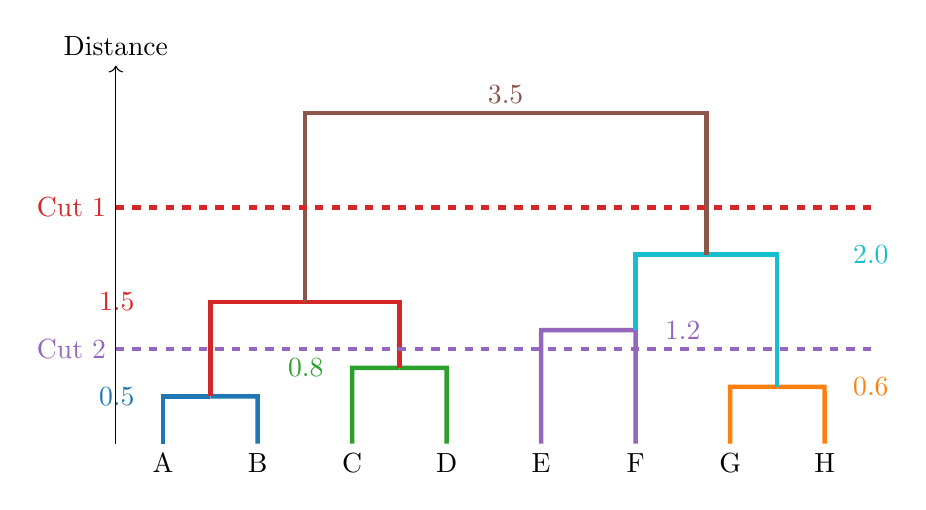
\begin{tikzpicture}[scale=1.2]
% Draw dendrogram
\coordinate (A) at (0,0);
\coordinate (B) at (1,0);
\coordinate (C) at (2,0);
\coordinate (D) at (3,0);
\coordinate (E) at (4,0);
\coordinate (F) at (5,0);
\coordinate (G) at (6,0);
\coordinate (H) at (7,0);

% Labels
\node[below] at (A) {A};
\node[below] at (B) {B};
\node[below] at (C) {C};
\node[below] at (D) {D};
\node[below] at (E) {E};
\node[below] at (F) {F};
\node[below] at (G) {G};
\node[below] at (H) {H};

% First merges
\draw[mlblue, ultra thick] (A) -- (0,0.5) -- (0.5,0.5) -- (0.5,0.5);
\draw[mlblue, ultra thick] (B) -- (1,0.5) -- (0.5,0.5);
\node[mlblue, left] at (-0.2,0.5) {0.5};

\draw[mlgreen, ultra thick] (C) -- (2,0.8) -- (2.5,0.8) -- (2.5,0.8);
\draw[mlgreen, ultra thick] (D) -- (3,0.8) -- (2.5,0.8);
\node[mlgreen, left] at (1.8,0.8) {0.8};

\draw[mlorange, ultra thick] (G) -- (6,0.6) -- (6.5,0.6) -- (6.5,0.6);
\draw[mlorange, ultra thick] (H) -- (7,0.6) -- (6.5,0.6);
\node[mlorange, right] at (7.2,0.6) {0.6};

% Second merges
\draw[mlred, ultra thick] (0.5,0.5) -- (0.5,1.5) -- (1.5,1.5);
\draw[mlred, ultra thick] (2.5,0.8) -- (2.5,1.5) -- (1.5,1.5);
\node[mlred, left] at (-0.2,1.5) {1.5};

\draw[mlpurple, ultra thick] (E) -- (4,1.2) -- (5,1.2);
\draw[mlpurple, ultra thick] (F) -- (5,1.2);
\node[mlpurple] at (5.5,1.2) {1.2};

% Third merge
\draw[mlcyan, ultra thick] (5,1.2) -- (5,2.0) -- (5.75,2.0);
\draw[mlcyan, ultra thick] (6.5,0.6) -- (6.5,2.0) -- (5.75,2.0);
\node[mlcyan, right] at (7.2,2.0) {2.0};

% Final merge
\draw[mlbrown, ultra thick] (1.5,1.5) -- (1.5,3.5) -- (3.625,3.5);
\draw[mlbrown, ultra thick] (5.75,2.0) -- (5.75,3.5) -- (3.625,3.5);
\node[mlbrown, above] at (3.625,3.5) {3.5};

% Cut lines
\draw[mlred, dashed, ultra thick] (-0.5,2.5) -- (7.5,2.5);
\node[mlred, left] at (-0.5,2.5) {Cut 1};

\draw[mlpurple, dashed, ultra thick] (-0.5,1.0) -- (7.5,1.0);
\node[mlpurple, left] at (-0.5,1.0) {Cut 2};

% Axis
\draw[->] (-0.5,0) -- (-0.5,4) node[above] {Distance};
\end{tikzpicture}
\end{center}

\vspace{0.5em}

\section*{Three Linkage Methods: Different Stories}

\begin{center}
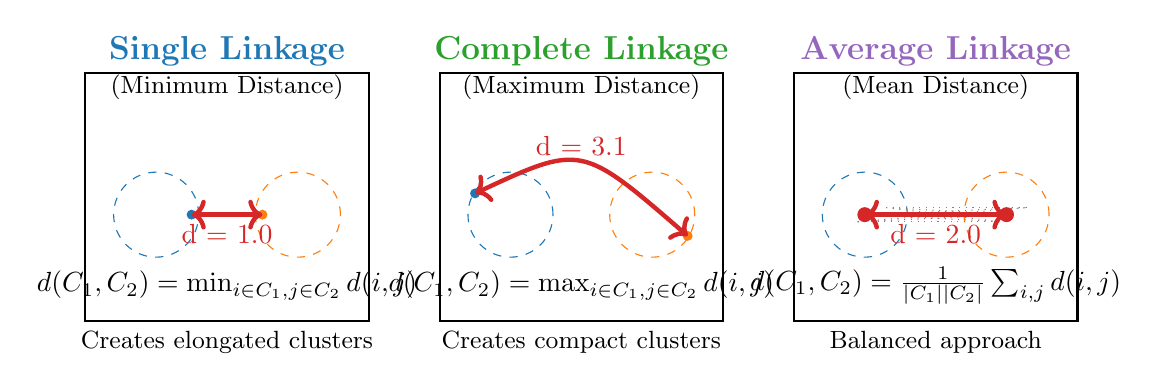
\begin{tikzpicture}[scale=0.9]
% Single linkage
\begin{scope}[shift={(0,0)}]
\draw[thick] (0,0) rectangle (4,3.5);
\node[font=\large\bfseries, mlblue] at (2,3.8) {Single Linkage};
\node[font=\small] at (2,3.3) {(Minimum Distance)};

% Two clusters
\draw[mlblue, dashed] (1,1.5) circle (0.6);
\draw[mlorange, dashed] (3,1.5) circle (0.6);

% Show minimum distance
\fill[mlblue] (1.5,1.5) circle (2pt);
\fill[mlorange] (2.5,1.5) circle (2pt);
\draw[mlred, ultra thick, <->] (1.5,1.5) -- (2.5,1.5);
\node[mlred, below] at (2,1.5) {d = 1.0};

% Formula
\node at (2,0.5) {$d(C_1,C_2) = \min_{i \in C_1, j \in C_2} d(i,j)$};
\node[below, font=\small] at (2,0) {Creates elongated clusters};
\end{scope}

% Complete linkage
\begin{scope}[shift={(5,0)}]
\draw[thick] (0,0) rectangle (4,3.5);
\node[font=\large\bfseries, mlgreen] at (2,3.8) {Complete Linkage};
\node[font=\small] at (2,3.3) {(Maximum Distance)};

% Two clusters
\draw[mlblue, dashed] (1,1.5) circle (0.6);
\draw[mlorange, dashed] (3,1.5) circle (0.6);

% Show maximum distance
\fill[mlblue] (0.5,1.8) circle (2pt);
\fill[mlorange] (3.5,1.2) circle (2pt);
\draw[mlred, ultra thick, <->] (0.5,1.8) .. controls (2,2.5) .. (3.5,1.2);
\node[mlred, above] at (2,2.2) {d = 3.1};

% Formula
\node at (2,0.5) {$d(C_1,C_2) = \max_{i \in C_1, j \in C_2} d(i,j)$};
\node[below, font=\small] at (2,0) {Creates compact clusters};
\end{scope}

% Average linkage
\begin{scope}[shift={(10,0)}]
\draw[thick] (0,0) rectangle (4,3.5);
\node[font=\large\bfseries, mlpurple] at (2,3.8) {Average Linkage};
\node[font=\small] at (2,3.3) {(Mean Distance)};

% Two clusters
\draw[mlblue, dashed] (1,1.5) circle (0.6);
\draw[mlorange, dashed] (3,1.5) circle (0.6);

% Show multiple distances
\foreach \i in {1,...,3} {
    \foreach \j in {1,...,3} {
        \draw[gray, dotted] (0.7+\i*0.2,1.3+\i*0.1) -- (2.7+\j*0.2,1.3+\j*0.1);
    }
}

% Centers
\fill[mlred] (1,1.5) circle (3pt);
\fill[mlred] (3,1.5) circle (3pt);
\draw[mlred, ultra thick, <->] (1,1.5) -- (3,1.5);
\node[mlred, below] at (2,1.5) {d = 2.0};

% Formula
\node at (2,0.5) {$d(C_1,C_2) = \frac{1}{|C_1||C_2|}\sum_{i,j} d(i,j)$};
\node[below, font=\small] at (2,0) {Balanced approach};
\end{scope}
\end{tikzpicture}
\end{center}

\newpage

\section*{Agglomerative vs Divisive: Two Strategies}

\begin{center}
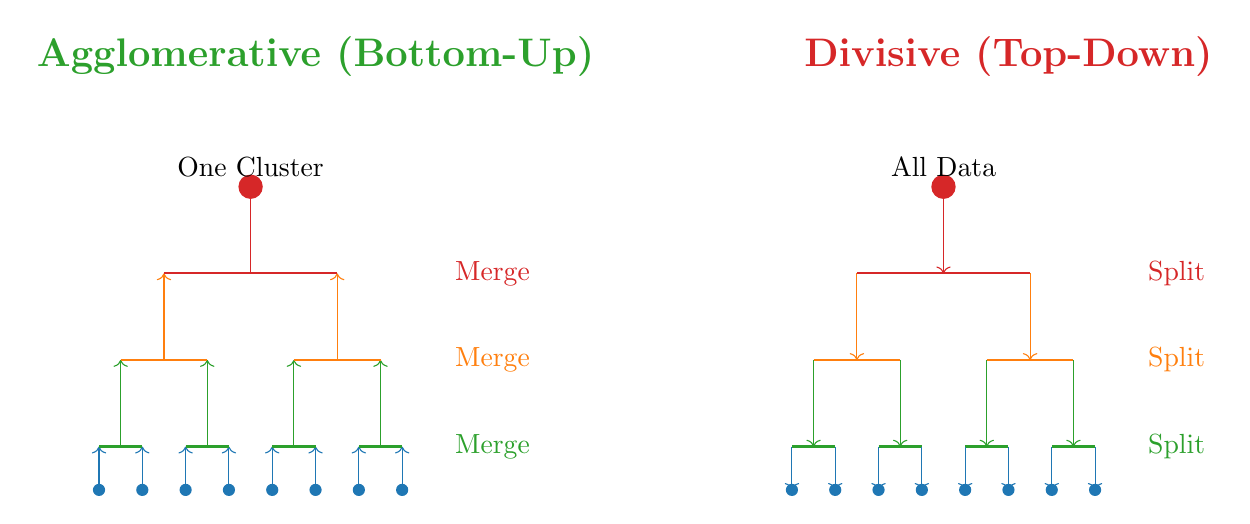
\begin{tikzpicture}[scale=1.1]
% Agglomerative (bottom-up)
\begin{scope}[shift={(0,0)}]
\node[font=\Large\bfseries, mlgreen] at (3,5) {Agglomerative (Bottom-Up)};

% Individual points at bottom
\foreach \i in {1,...,8} {
    \fill[mlblue] (0.5*\i,0) circle (2pt);
    \draw[mlblue, ->] (0.5*\i,0) -- (0.5*\i,0.5);
}

% First merge level
\draw[mlgreen, thick] (0.5,0.5) -- (1,0.5);
\draw[mlgreen, thick] (1.5,0.5) -- (2,0.5);
\draw[mlgreen, thick] (2.5,0.5) -- (3,0.5);
\draw[mlgreen, thick] (3.5,0.5) -- (4,0.5);

\draw[mlgreen, ->] (0.75,0.5) -- (0.75,1.5);
\draw[mlgreen, ->] (1.75,0.5) -- (1.75,1.5);
\draw[mlgreen, ->] (2.75,0.5) -- (2.75,1.5);
\draw[mlgreen, ->] (3.75,0.5) -- (3.75,1.5);

% Second merge level
\draw[mlorange, thick] (0.75,1.5) -- (1.75,1.5);
\draw[mlorange, thick] (2.75,1.5) -- (3.75,1.5);

\draw[mlorange, ->] (1.25,1.5) -- (1.25,2.5);
\draw[mlorange, ->] (3.25,1.5) -- (3.25,2.5);

% Final merge
\draw[mlred, thick] (1.25,2.5) -- (3.25,2.5);
\draw[mlred, ->] (2.25,2.5) -- (2.25,3.5);

\fill[mlred] (2.25,3.5) circle (4pt);
\node[above] at (2.25,3.5) {One Cluster};

\node[mlgreen, right] at (4.5,0.5) {Merge};
\node[mlorange, right] at (4.5,1.5) {Merge};
\node[mlred, right] at (4.5,2.5) {Merge};
\end{scope}

% Divisive (top-down)
\begin{scope}[shift={(8,0)}]
\node[font=\Large\bfseries, mlred] at (3,5) {Divisive (Top-Down)};

% One cluster at top
\fill[mlred] (2.25,3.5) circle (4pt);
\node[above] at (2.25,3.5) {All Data};
\draw[mlred, ->] (2.25,3.5) -- (2.25,2.5);

% First split
\draw[mlred, thick] (1.25,2.5) -- (3.25,2.5);
\draw[mlorange, ->] (1.25,2.5) -- (1.25,1.5);
\draw[mlorange, ->] (3.25,2.5) -- (3.25,1.5);

% Second split
\draw[mlorange, thick] (0.75,1.5) -- (1.75,1.5);
\draw[mlorange, thick] (2.75,1.5) -- (3.75,1.5);

\draw[mlgreen, ->] (0.75,1.5) -- (0.75,0.5);
\draw[mlgreen, ->] (1.75,1.5) -- (1.75,0.5);
\draw[mlgreen, ->] (2.75,1.5) -- (2.75,0.5);
\draw[mlgreen, ->] (3.75,1.5) -- (3.75,0.5);

% Final split
\draw[mlgreen, thick] (0.5,0.5) -- (1,0.5);
\draw[mlgreen, thick] (1.5,0.5) -- (2,0.5);
\draw[mlgreen, thick] (2.5,0.5) -- (3,0.5);
\draw[mlgreen, thick] (3.5,0.5) -- (4,0.5);

% Individual points
\foreach \i in {1,...,8} {
    \fill[mlblue] (0.5*\i,0) circle (2pt);
    \draw[mlblue, ->] (0.5*\i,0.5) -- (0.5*\i,0);
}

\node[mlred, right] at (4.5,2.5) {Split};
\node[mlorange, right] at (4.5,1.5) {Split};
\node[mlgreen, right] at (4.5,0.5) {Split};
\end{scope}
\end{tikzpicture}
\end{center}

\vspace{1em}

\section*{Distance Matrix: The Foundation}

\begin{center}
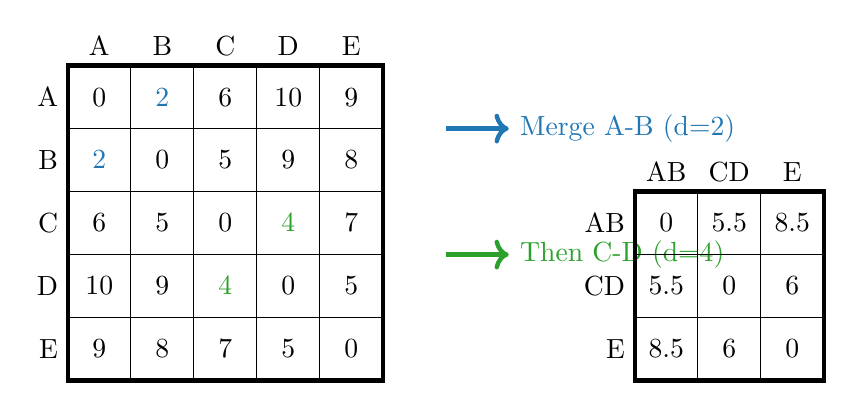
\begin{tikzpicture}[scale=0.8]
% Distance matrix
\draw[ultra thick] (0,0) rectangle (5,5);
\foreach \i in {1,...,4} {
    \draw (0,\i) -- (5,\i);
    \draw (\i,0) -- (\i,5);
}

% Labels
\node[left] at (0,4.5) {A};
\node[left] at (0,3.5) {B};
\node[left] at (0,2.5) {C};
\node[left] at (0,1.5) {D};
\node[left] at (0,0.5) {E};

\node[above] at (0.5,5) {A};
\node[above] at (1.5,5) {B};
\node[above] at (2.5,5) {C};
\node[above] at (3.5,5) {D};
\node[above] at (4.5,5) {E};

% Values
\node at (0.5,4.5) {0};
\node[mlblue] at (1.5,4.5) {2};
\node at (2.5,4.5) {6};
\node at (3.5,4.5) {10};
\node at (4.5,4.5) {9};

\node[mlblue] at (0.5,3.5) {2};
\node at (1.5,3.5) {0};
\node at (2.5,3.5) {5};
\node at (3.5,3.5) {9};
\node at (4.5,3.5) {8};

\node at (0.5,2.5) {6};
\node at (1.5,2.5) {5};
\node at (2.5,2.5) {0};
\node[mlgreen] at (3.5,2.5) {4};
\node at (4.5,2.5) {7};

\node at (0.5,1.5) {10};
\node at (1.5,1.5) {9};
\node[mlgreen] at (2.5,1.5) {4};
\node at (3.5,1.5) {0};
\node at (4.5,1.5) {5};

\node at (0.5,0.5) {9};
\node at (1.5,0.5) {8};
\node at (2.5,0.5) {7};
\node at (3.5,0.5) {5};
\node at (4.5,0.5) {0};

% Arrows showing minimum
\draw[mlblue, ultra thick, ->] (6,4) -- (7,4) node[right] {Merge A-B (d=2)};
\draw[mlgreen, ultra thick, ->] (6,2) -- (7,2) node[right] {Then C-D (d=4)};

% Updated matrix
\begin{scope}[shift={(9,0)}]
\draw[ultra thick] (0,0) rectangle (3,3);
\foreach \i in {1,2} {
    \draw (0,\i) -- (3,\i);
    \draw (\i,0) -- (\i,3);
}

\node[left] at (0,2.5) {AB};
\node[left] at (0,1.5) {CD};
\node[left] at (0,0.5) {E};

\node[above] at (0.5,3) {AB};
\node[above] at (1.5,3) {CD};
\node[above] at (2.5,3) {E};

\node at (0.5,2.5) {0};
\node at (1.5,2.5) {5.5};
\node at (2.5,2.5) {8.5};

\node at (0.5,1.5) {5.5};
\node at (1.5,1.5) {0};
\node at (2.5,1.5) {6};

\node at (0.5,0.5) {8.5};
\node at (1.5,0.5) {6};
\node at (2.5,0.5) {0};
\end{scope}
\end{tikzpicture}
\end{center}

\vspace{1em}

\section*{Discovery Challenge: Build Your Tree}

\begin{center}
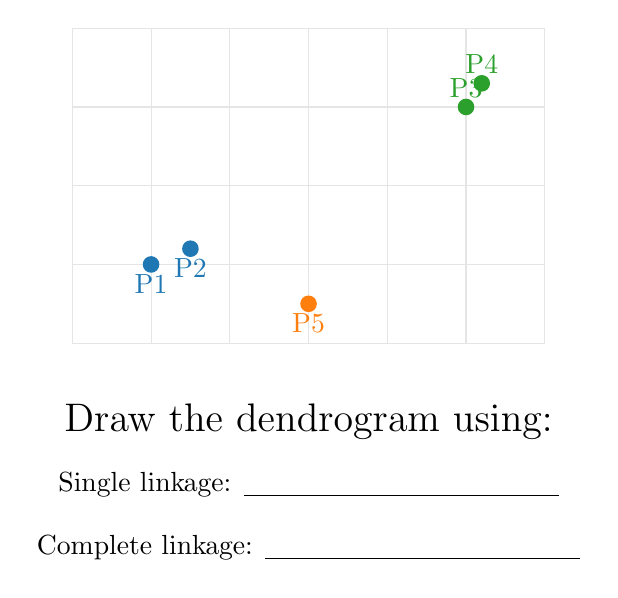
\begin{tikzpicture}[scale=1]
% Points to cluster
\draw[gray!20] (0,0) grid (6,4);
\fill[mlblue] (1,1) circle (3pt) node[below] {P1};
\fill[mlblue] (1.5,1.2) circle (3pt) node[below] {P2};
\fill[mlgreen] (5,3) circle (3pt) node[above] {P3};
\fill[mlgreen] (5.2,3.3) circle (3pt) node[above] {P4};
\fill[mlorange] (3,0.5) circle (3pt) node[below] {P5};

\node[font=\Large] at (3,-1) {Draw the dendrogram using:};
\node at (3,-1.8) {Single linkage: \underline{\hspace{4cm}}};
\node at (3,-2.6) {Complete linkage: \underline{\hspace{4cm}}};
\end{tikzpicture}
\end{center}

\vspace{0.5em}

\begin{tcolorbox}[colback=mlcyan!10, colframe=mlcyan!50]
\centering\large
\textbf{Key Insight:} No need to choose k - cut the tree at any height!
\end{tcolorbox}

\end{document}